\section{The Current Situation}\label{sec:the-current-situation}

Several shortcomings from NOVA have been documented in the transcript below.
The most noticeable is the issues regarding the~\acrfull{epos} insights and how they are not elaborate enough in its
current state.

\blockquote[Paraphrased from an interview with Nancy, owner of NOVA]{As NOVA is a relatively new business, many minor
issues, as well as major issues, have to be solved.
We are lacking~\acrshort{bi} both because we are a new business, but also because our current~\acrshort{epos} does not
allow for sufficient insights into our data.

A consequence of this is that we do not know how effective our loyalty program is.
Moreover, the~\acrshort{epos} only provides sales data at a daily level and not an hourly level.
This makes for unnecessary difficulty understanding when throughout the day the business is most busy and thereby makes
it difficult to efficiently allocate human resources.
In addition, we do not know when in the day certain products are sold and thereby cannot effectively prepare said
products efficiently.

For us, the most important requirement of a potential solution is that it has to be user-friendly for all personnel —
both technically and non-technically proficient.}

From the interview, the authors chose to focus on two of the primary concerns identified by Nancy.
The first problem can be seen visualized through a rich picture as seen in Figure~\ref{fig:pda-scheduling-problem}.
% textidote: ignore begin
\begin{figure}[H]
    \centering
    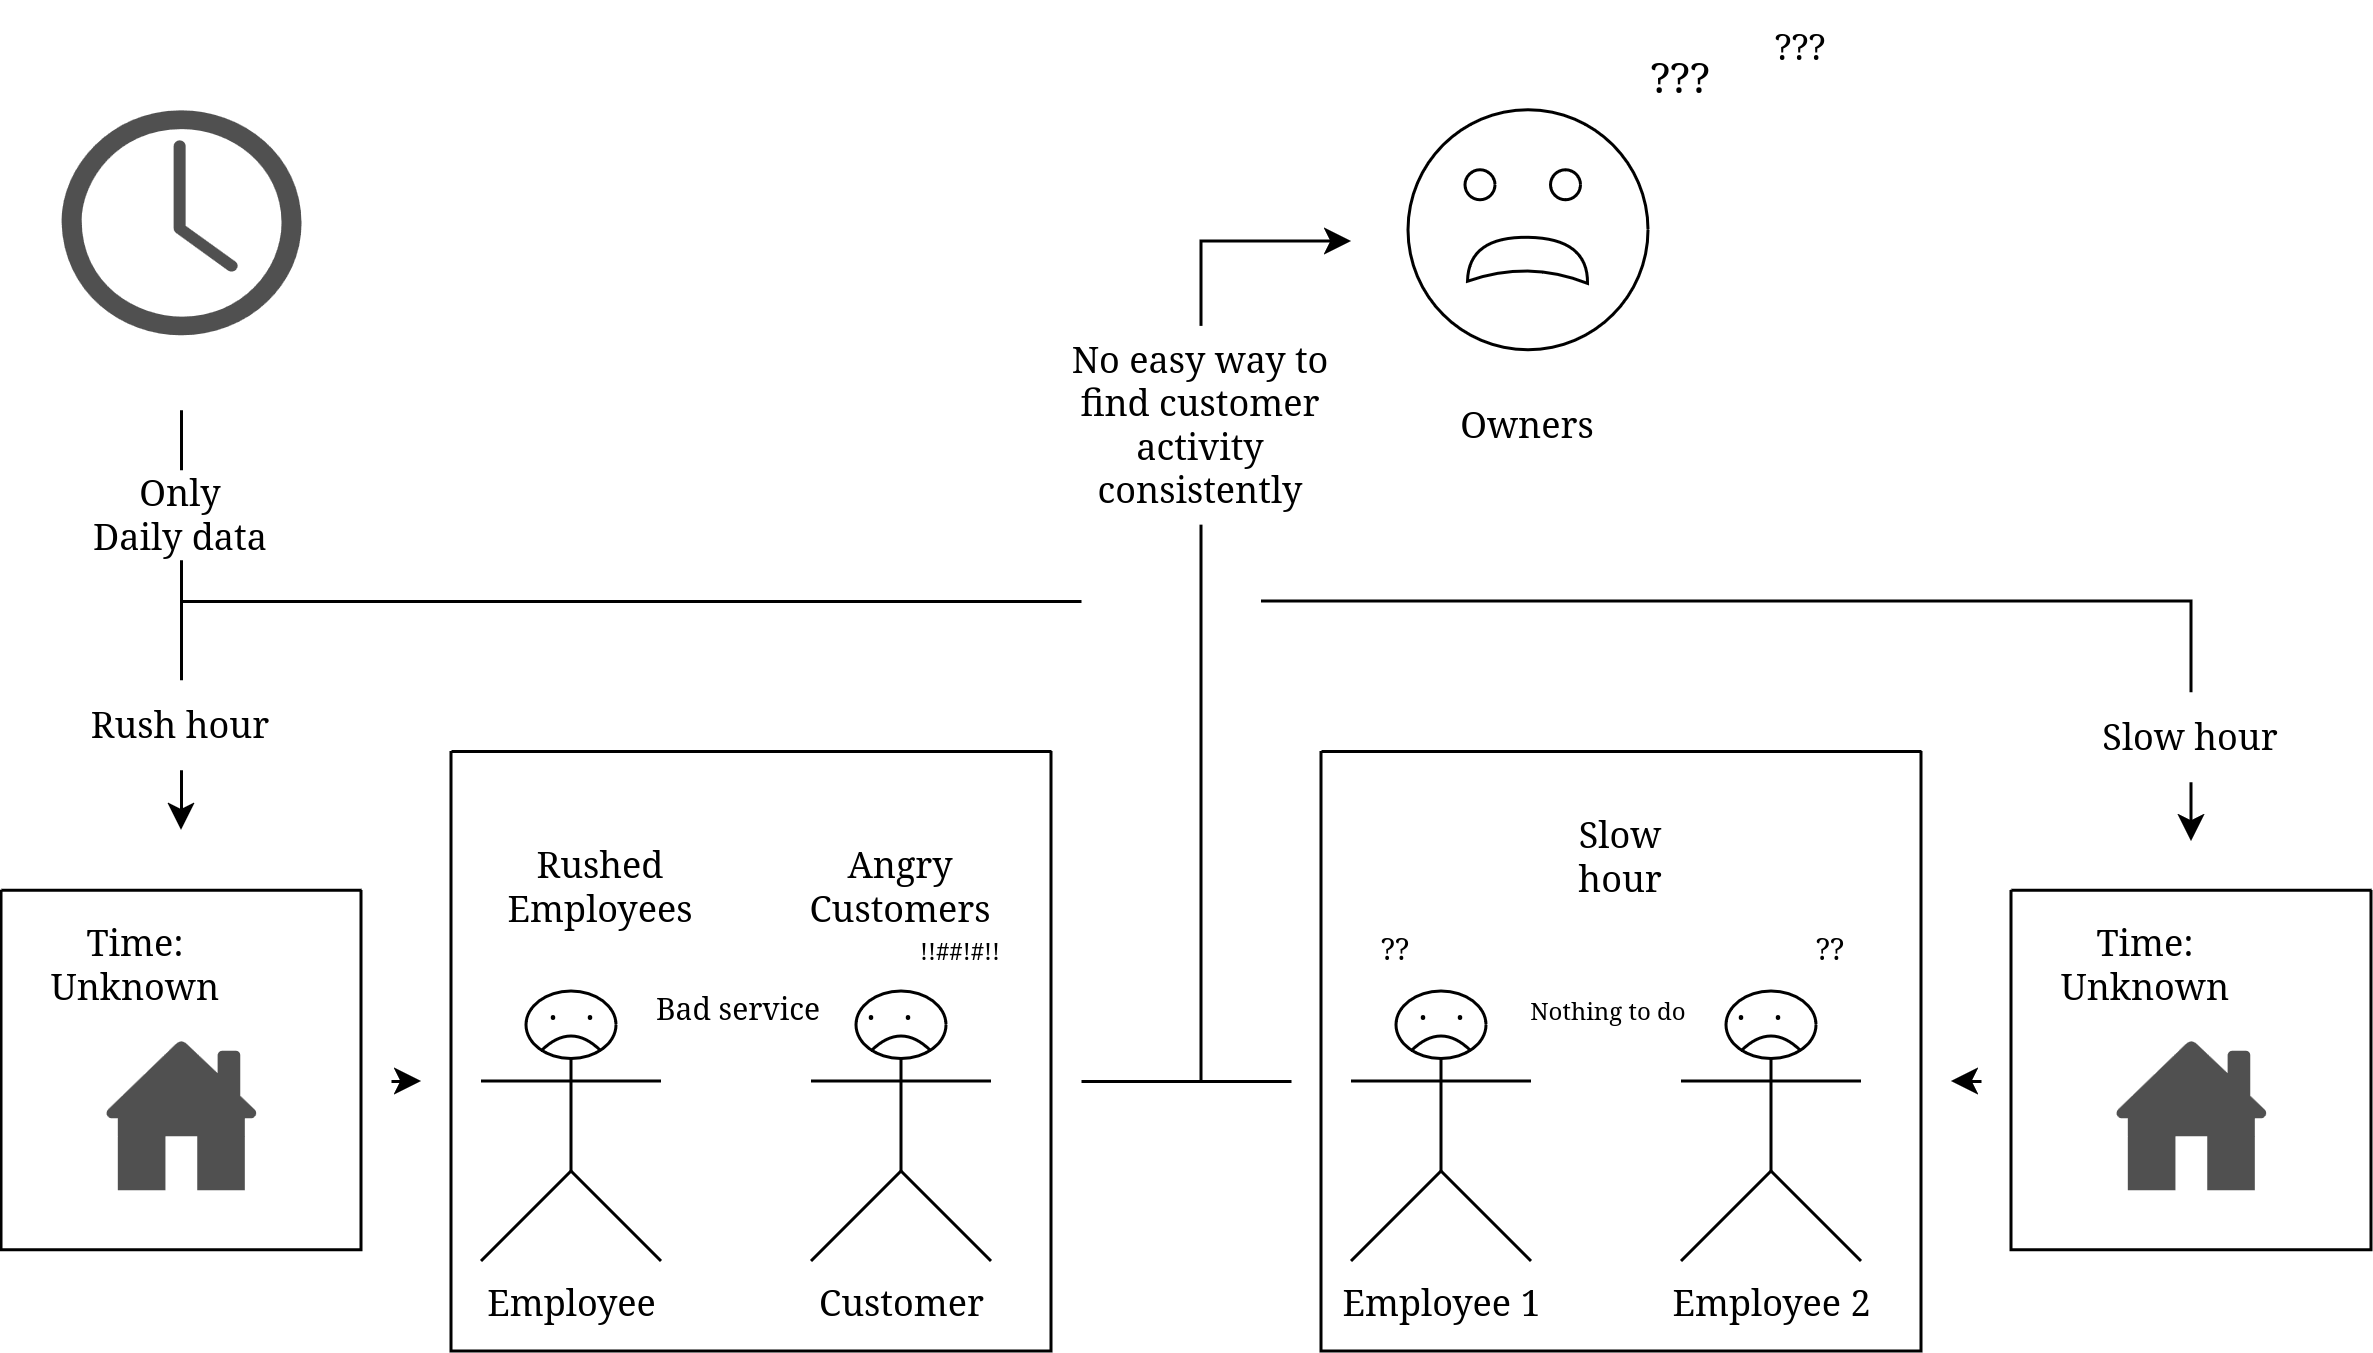
\includegraphics[width=\textwidth]{rich_pictures_scheduling}
    \caption{Rich picture of the scheduling problem Nova café has.}\label{fig:pda-scheduling-problem}
\end{figure}
% textidote: ignore end
The figure depicts the likely outcomes of Nova not having hourly data about their customer activity,
which can likely end in bad customer service or the employee's not having enough work for multiple people.

The other issue that the authors will focus on solving for Nova is their food management difficulties.
Without detailed data on when specific items are sold, and in what quantity, it is challenging to plan
for when and how much they should make of their food products.
This can result in a large quantity of food having to be thrown out.
The inverse could also happen, which would be Nova selling out on popular products which stops them
from servicing customers.
This problem is visualized in Figure~\ref{fig:pda-waste-problem}.

% textidote: ignore begin
\begin{figure}[H]
    \centering
    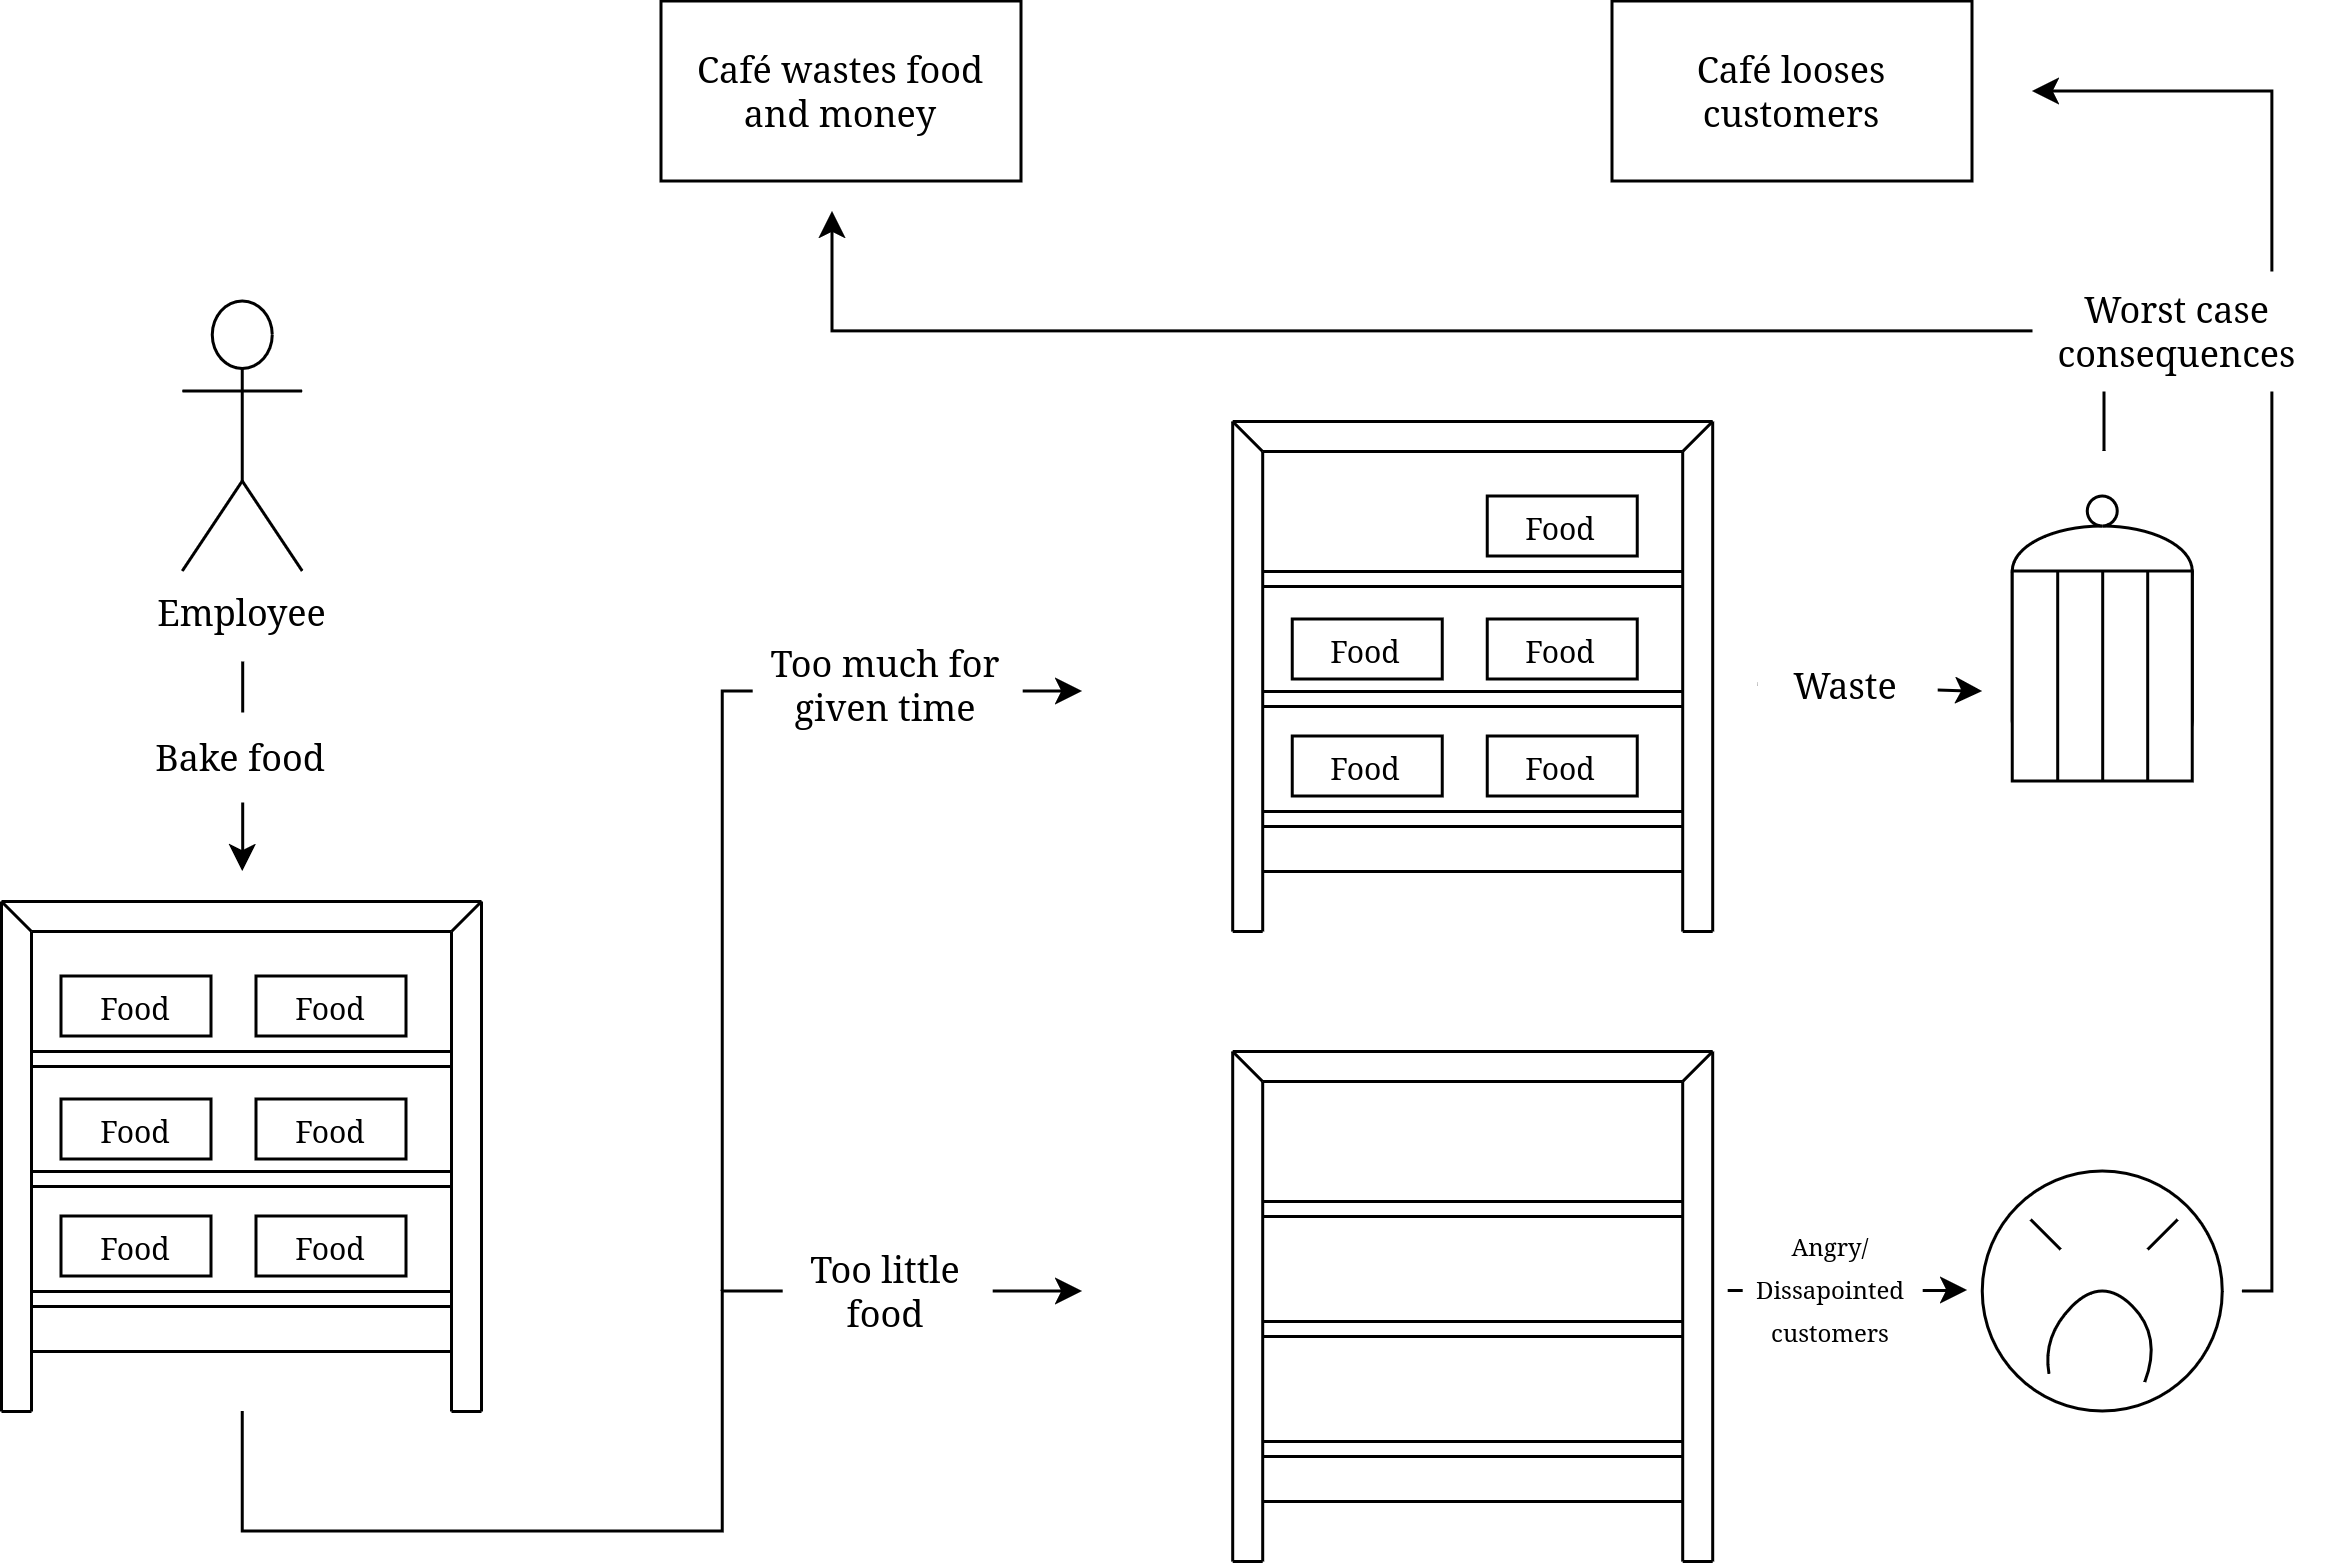
\includegraphics[width=\textwidth]{rich_pictures_waste}
    \caption{Rich picture of the food waste problem Nova café has.}\label{fig:pda-waste-problem}
\end{figure}
% textidote: ignore end
